\documentclass{article}

\usepackage{amsmath}
\usepackage{amssymb}
\usepackage{geometry}
\usepackage{graphicx}
\usepackage{minted}
\usepackage[shortlabels]{enumitem}
\usepackage[style=ieee, url=false]{biblatex}
\addbibresource{bibliography/jetpump.bib}
\usepackage{float}
\usepackage{commath}

% Make header with name and date etc.
\usepackage{fancyhdr}
\lhead{Kaelin Ellis\\Math F661: Optimization}
\rhead{\today\\Project Working}
\pagestyle{fancy}

\usepackage[utf8]{inputenc}
\setlength{\parindent}{0pt} % Don't indent new paragraphs
\setlength{\headheight}{24pt} 

% Import titlesec package for customizing section titles
\usepackage{titlesec}

% Redefine \section to be non-bold and without numbers
\titleformat{\section}
  {\bfseries\large} % Bold font (\bfseries) and large size
  {} % No numbering
  {0pt} % No extra spacing
  {} % No special formatting before section title

\begin{document}

\begin{center}
    \Large Title: Optimizing Power Fluid in Jet Pumps \par
\end{center}

\section{Introduction}

The proposed project is application driven. Oil wells on jet pumps have to share a common resource called power fluid to assist with lifting the well to surface. If the power fluid is unlimited, then an unconstrained optimization problem exists and each well can be lifted with the max power fluid required. In mature fields with many wells, this is not the condition, and the wells are required to share a finite resource of power fluid. As such an optimization scheme needs to be developed to appropriately divide the power fluid to maximize oil production. A network overview of four wells sharing power fluid from a common kinetic pump is shown in figure \ref{fig:jetpump_network}.

\begin{figure}[H]
    \centering
    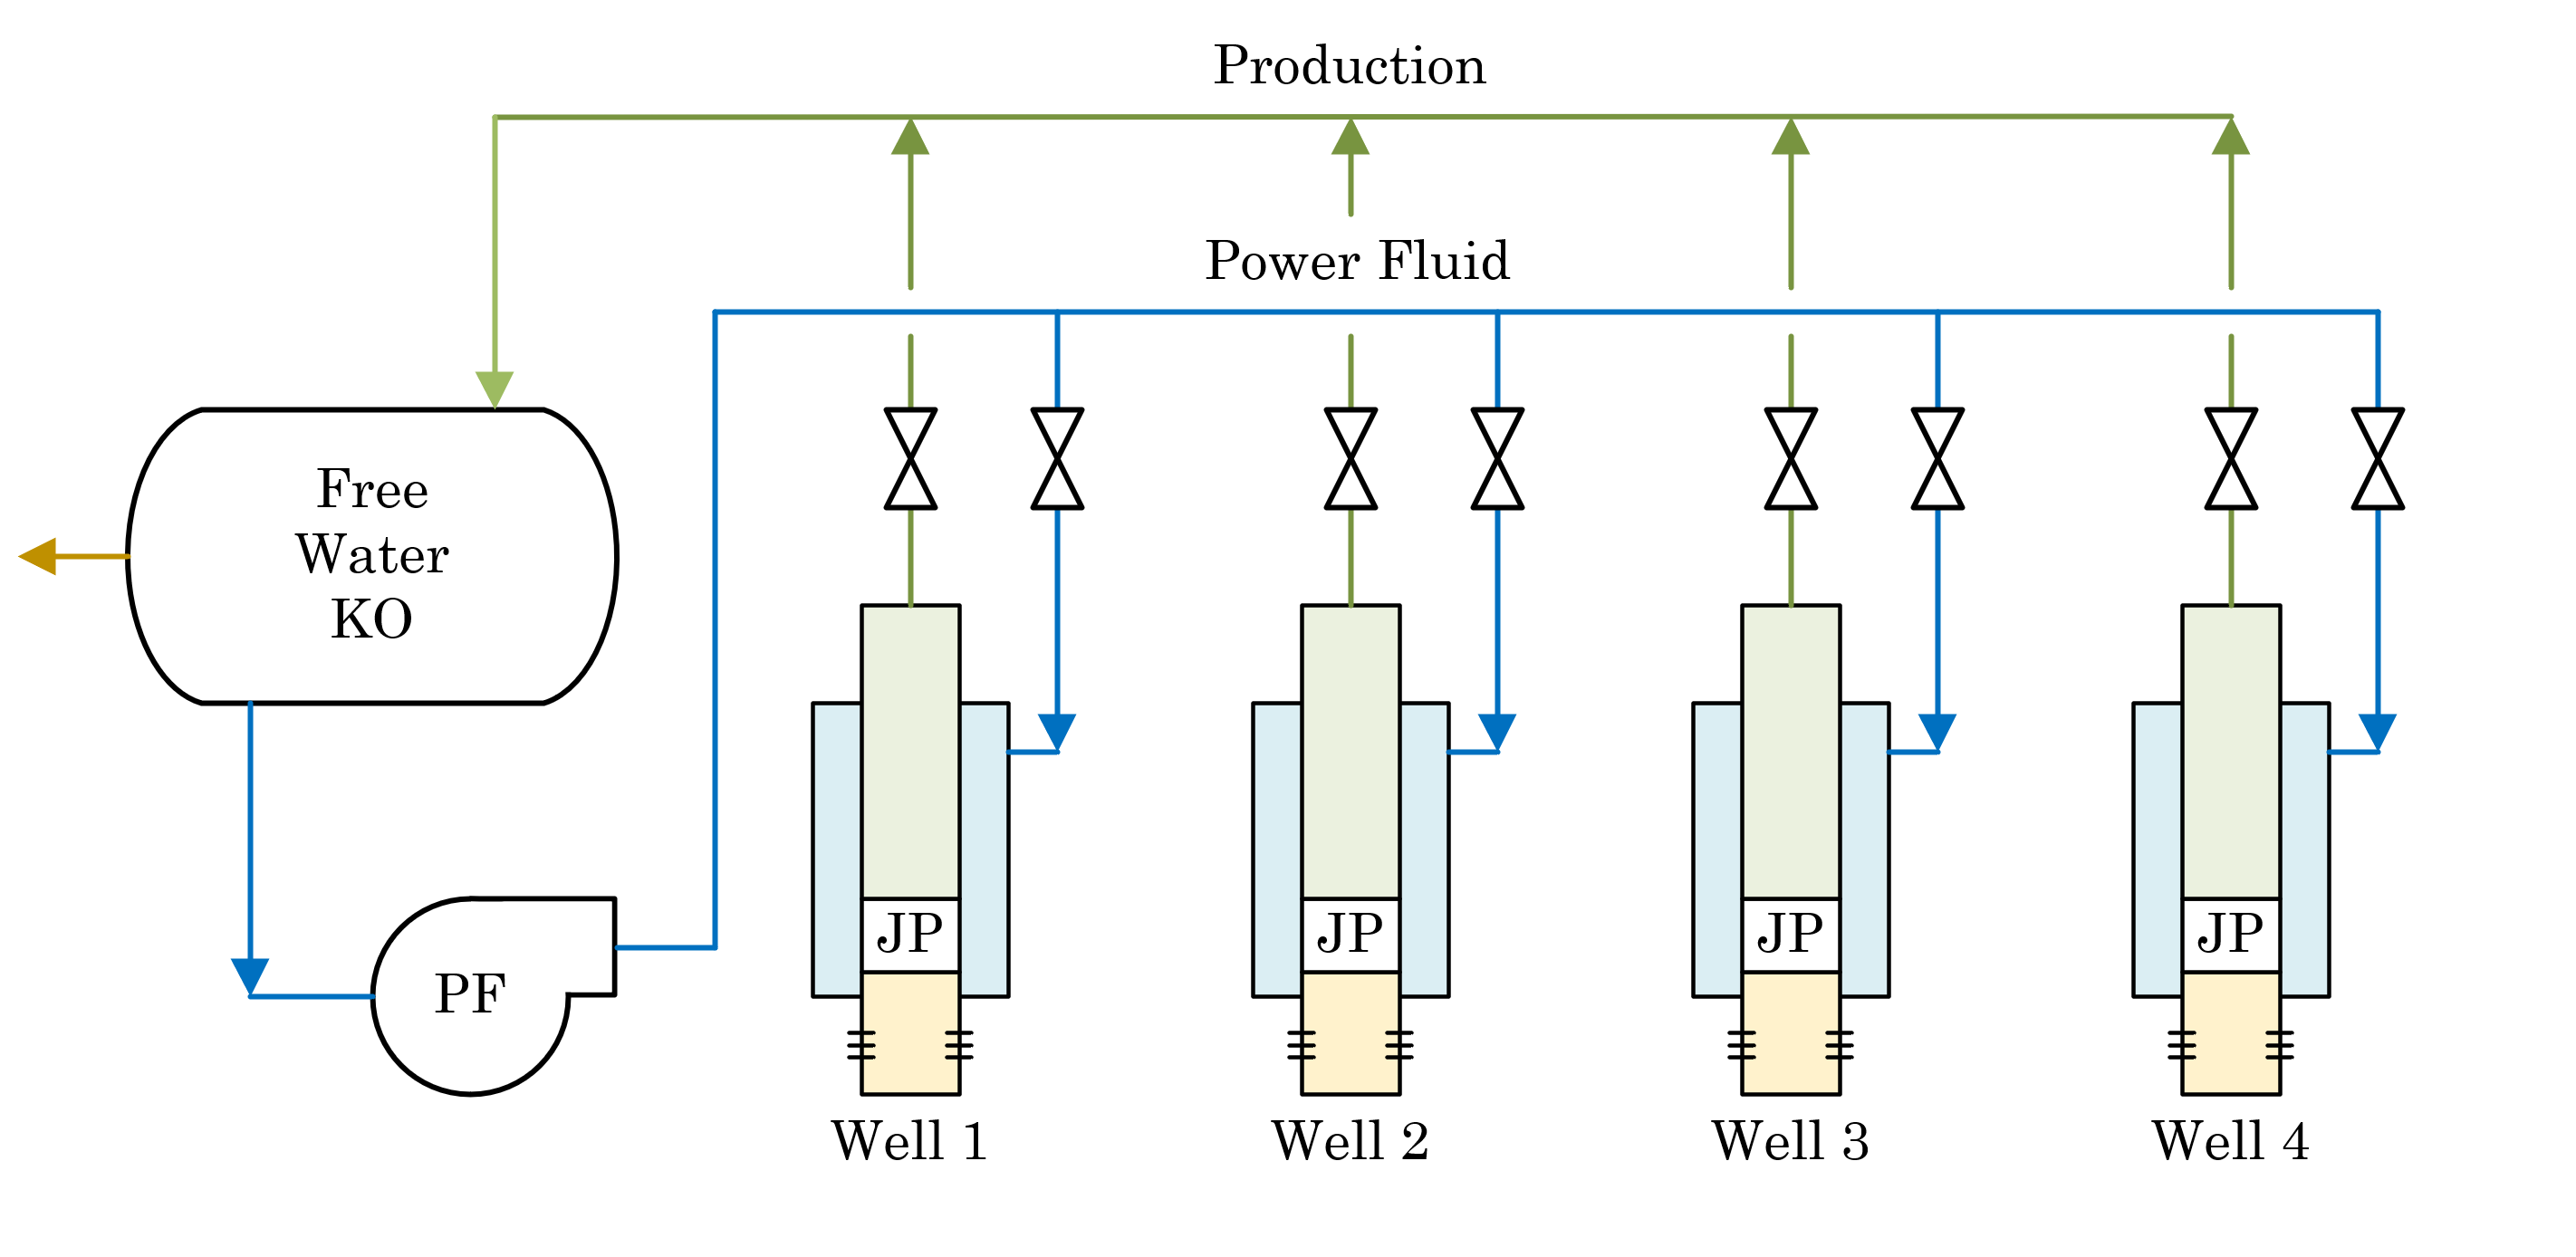
\includegraphics[width=1\linewidth]{figures/network_diagram.PNG}
    \caption{Network Diagram of Four Wells}
    \label{fig:jetpump_network}
\end{figure}

\section{Mathematical Model}

The oil production from a well on jet pump is represented with the equation below. Where $q_{o}$ is the oil produced and $q_{p}$ is the power fluid volume required.

\begin{equation*}
    q_{oi} = c_{1i} - c_{2i} \exp{(-q_{pi} c_{3i})}
\end{equation*}

The coefficients $c_{1}$, $c_{2}$ and $c_{3}$ for each well are found in a separate numerical scheme and are dependent on the specific wells water cut, formation gas oil ratio and specific subsurface geometry. The optimization objective function and constraints are as follows:

\begin{equation*}
\begin{aligned}
    \text{maximize } & Q_{o} = \sum_{i=1}^{n} q_{o\:i} = f(Q_{p}) \\
    \text{subject to } & Q_{p} = \sum_{i=1}^{n} q_{p\:i} \leq Q_{\text{p}}^{\text{tot}} \\
    & q_{p\:i} \geq 0 \\
\end{aligned}
\end{equation*}

The index $i$ represents a specific unique oil well that is on the network.

\section{Network Example}

To assist with understand the basic ideas and mathematics, an example will network will be created with 3 wells to demonstrate. The well model takes the form of the form of

\begin{equation*}
\begin{aligned}
    q_{o1} = & c_{11} - c_{21} \exp{(-q_{p1} c_{31})} \\
    q_{o2} = & c_{12} - c_{22} \exp{(-q_{p2} c_{32})} \\
    q_{o3} = & c_{13} - c_{23} \exp{(-q_{p3} c_{33})}
\end{aligned}
\end{equation*}

The objective function takes the following form:

\begin{equation*}
\begin{aligned}
    Q_{o} = & q_{o1} + q_{o2} +  q_{o3}\\
    Q_{o} = & c_{11} - c_{21} \exp{(-q_{p1} c_{31})} + c_{12} - c_{22} \exp{(-q_{p2} c_{32})} + c_{13} - c_{23} \exp{(-q_{p3} c_{33})}
\end{aligned}
\end{equation*}

The individual wells first and second partial derivative with respect to its individual power fluid takes the following form.

\begin{equation*}
\begin{aligned}
    \dfrac{\partial oi}{\partial pi} & = - c_{2i} c_{3i} \exp{(-q_{pi} c_{3i})} \\
    \dfrac{\partial^{2} oi}{\partial pi \partial pi} & = - c_{2i} c_{3i}^{2} \exp{(-q_{pi} c_{3i})} \\
\end{aligned}
\end{equation*}

The gradient of the objective function appears as the following:

\begin{equation*}
    \nabla Q_{o} = 
    \begin{pmatrix}
    - c_{21} c_{31} \exp{(-q_{p1} c_{31})} \\[6pt]
    - c_{22} c_{32} \exp{(-q_{p2} c_{32})} \\[6pt]
    - c_{23} c_{33} \exp{(-q_{p3} c_{33})} 
    \end{pmatrix}
\end{equation*}

The Hessian is straight forward if Newton's method was desired to be used.

\begin{equation*}
    \nabla^{2} Q_{o} = 
    \begin{pmatrix}
    - c_{21} c_{31}^{2} \exp{(-q_{p1} c_{31})} & 0 & 0 \\[6pt]
    0 & - c_{22} c_{32}^{2} \exp{(-q_{p2} c_{32})} & 0 \\[6pt]
    0 & 0 & - c_{23} c_{33}^{2} \exp{(-q_{p3} c_{33})} 
    \end{pmatrix}
\end{equation*}

\section{Network Constraint Example}

Incorporating constraints from the defined example of three oil wells. The power fluid sent to each well is represented by a 3-dimensional column vector that takes the following form.

\begin{equation*}
    Q_{p} = 
    \begin{pmatrix}
    q_{p1} \\
    q_{p2} \\
    q_{p3} 
    \end{pmatrix}
\end{equation*}

Reading the paper and thesis by Nobu it appears that makes $n+1$ linear equalities. The system of linear inequalities takes the following form.

\begin{equation*}
    Q_{p}^{T}n_{i} - b_{i} \geq 0 
\end{equation*}

Where $n_{i}$ are n-dimensional column vectors. Which will all sum to one. The first column and entry in the matrix accounts for the fact that the total water has to be less than the available supply. (I am not sure why you need a negative sign).

\begin{equation*}
    n_{0} = 
    \begin{pmatrix}
    -\dfrac{1}{\sqrt{3}} \\[10pt]
    -\dfrac{1}{\sqrt{3}} \\[10pt]
    -\dfrac{1}{\sqrt{3}}
    \end{pmatrix} \:
    b_{0} = -\dfrac{Q_{p}^{tot}}{\sqrt{3}}
\end{equation*}

All the other entries in the matrix are for each individual wells flow. For the second well, this would take the following form.

\begin{equation*}
    n_{2} = 
    \begin{pmatrix}
    0 \\
    1 \\
    0
    \end{pmatrix} \:
    b_{2} = 0
\end{equation*}

A matrix is generated called $N_{q}$ that accounts for all the active constraints. For examples, lets say all the constraints are active in our system (which is impossible), the matrix $N_{q}$ would appear as $N_{q} = (n_{0}, n_{1}, n_{2}, n_{3})$. The vector $b_{q}$ is also detailed out below. Shown in detail below.

\begin{equation*}
    N_{q} = 
    \begin{pmatrix}
    -\dfrac{1}{\sqrt{3}} & 1 & 0 & 0 \\[10pt]
    -\dfrac{1}{\sqrt{3}} & 0 & 1 & 0\\[10pt]
    -\dfrac{1}{\sqrt{3}} & 0 & 0 & 1
    \end{pmatrix} \:
    b_{0} = 
    \begin{pmatrix}
    -\dfrac{Q_{p}^{tot}}{\sqrt{3}} \\[10pt]
    0 \\[10pt]
    0 \\[10pt]
    0
    \end{pmatrix}
\end{equation*}

With $N_{q}$ the constraints appear as the following: $N_{q}^{T}Q_{p} - b_{q} \geq 0$. In more reality, the only constraint that will most likely be active is the total pad constraint. For my project, trying to incorporate this projection matrix might be difficult?

\section{Bueler Constraint Method}

Ed recommends making the constraints disappear by saying that the power fluid has to be equal to the constraint.

\begin{equation*}
    Q_{p} = \sum_{i=1}^{n} q_{p\:i} = Q_{\text{p}}^{\text{tot}}
\end{equation*}

You can eliminate one of the variables. In this case, we return to the 3 well network example. The third well power fluid will be written as $q_{p3} = Q_{p}^{tot} - q_{p1} - q_{p2}$. Then $Q_{p} = (q_{p1}, q_{p2})^{T}$. My only question here, is how do you ensure that $q_{p1}$ and $q_{p2}$ don't exceed $Q_{p}^{tot}$ and you end up with a negative $q_{p3}$? If you are doing unconstrained optimization, the first and second wells could select power fluid rates that are just way too high. Part of why this might happen, is because the function $q_{o} \approx \exp(q_{p})$ is not quadratic?

\section{Methodology Newton with Constraints}

Rough overview of this can be found on page 566 of the textbook.

\begin{enumerate}
    \item Set initial conditions:
    \begin{enumerate}
        \item k, iteration counter $k=0$
        \item $x_{0}$, power fluid for each well, even split to start
        \item $\nabla f(x_{0})$, Gradient
        \item $\nabla^2 f(x_{0})$, Hessian
    \end{enumerate}
    
    \item Active Constraints: Test what is active from $A$ and $b$ by whether it meets the equality condition, ensure none of the constraints are exceeded in the equality condition. 
    $$\bar{A} \text{ and } \bar{b}$$ 
    Note: the book goes from using $\hat{A}$ to $\bar{A}$ to define active inequality conditions. Uses $W$ to track indices of active constraints.
    
    \item Null Space and Lagrange Multipliers:
    
    Use QR factorization for matrices $Q_{1}$, $Q_{2}$, and $R_{1}$. Ref pg 91 and pg 559.

    \begin{equation*}
        A^T = QR = (Q_1 \: Q_2) \begin{pmatrix} R_1 \\ 0 \end{pmatrix}
    \end{equation*}
    
    \begin{enumerate}
        \item $\bar{Z}$ Null Space of $\bar{A}$
            $$Z = Q_{2}$$

        \item $\bar{\lambda}$ Lagrangian Multiples at active constraints.
        \begin{equation*}
        \begin{aligned}
            \bar{\lambda} & = \bar{A}^{T}_{r}\nabla f(x_{k}) \\
            A_{r} & = A^{T}(AA^{T})^{-1} \\
            \text{Where QR } & \text{is used} \\
            A_{r} & = Q_{1}R_{1}^{-T}
        \end{aligned}
        \end{equation*}
        \textit{Complementary Slackness} on Pg 496 implies inactive should be set to zero.
    \end{enumerate}
    
    \item Test for Optimality
    \begin{enumerate}
        \item If $\bar{Z}^{T}\nabla f(x_{k}) = 0$ and no constraints are active, you are optimal.
        \item If constraints are active (pg. 565): 
        \begin{enumerate}
            \item If $\bar{\lambda} \geq 0$ then stop, local stationary point has been reached
            \item If $\bar{\lambda} < 0$ drop a constraint. Update $W$, $\bar{A}$, $\bar{A_{r}}$ and $\bar{Z}$.
        \end{enumerate}
    \end{enumerate}

    \item Search Direction using Reduced Newton Method

    $$p = Zv = -Z(Z^{T}\nabla^2 f(x_k)Z)^{-1}Z^{T}\nabla f(x_{k})$$

    Reference Page 550 of the textbook.
    
    \item Step Size, $\alpha$.
    \begin{enumerate}
        \item Line search with backtracking. The book on page 378 gives a very simple algorithm for selecting alpha. Basically it is a guess and check method. Start with $\alpha = 1$ and see if $f(x_{k+1} < f(x_{k})$, if it is, stop. If not now $\alpha = \frac{1}{2}$. Check again, if not now, $\alpha = \frac{1}{4}$. Keep going using $\alpha_{i} = 2^{-i}$.
    \end{enumerate}
    
    \item Distance to inactive constraints. Defined as $\tau$ in thesis and $\bar{\alpha}$ in the book. Need to use the inactive constraints for the calculation. This is detailed out on Page 80 / 81 in the textbook.
    \begin{equation*}
        \bar{\alpha} = \min \left\{ \dfrac{a_i^T \bar{x} - b_{i}}{-a_i^T p} : a_i^T p < 0 \right \}
    \end{equation*}
    
    \item $\alpha = \min(\alpha, \bar{\alpha})$ said another way, $\alpha \leq \bar{\alpha}$.
    
    \item If $\alpha = \bar{\alpha}$ add the constraint. Update $W$, $\bar{A}$, $\bar{A_{r}}$ and $\bar{Z}$.

    \item Update $x_{k}$ by using $x_{k+1} = x_{k} + \alpha p$.
    
\end{enumerate}

\section{Methodology LMQN}

LMQN: Limited Memory Quasi Newton.

\begin{enumerate}
    \item Set initial conditions:
    \begin{enumerate}
        \item k, iteration counter $k=0$
        \item q, constraint counter $q=0$
        \item $x_{0}$, power fluid for each well, even split to start
        \item $\nabla f(x_{0})$, gradient
        \item $H_{0}^q = I$, set the LMQN matrix to the identity matrix
    \end{enumerate}
    
    \item Chose which constraints are active from $A$ and $b$ by testing whether it meets the equality condition, ensure none of the constraints are exceeded in the equality condition. 
    $$\bar{A} \text{ and } \bar{b}$$ 
    Note: the book goes from using $\hat{A}$ to $\bar{A}$ to define active inequality conditions. \\
    
    For any constraints that are active, add them into the LMQN that is approximated by the identity matrix using the following formula. The variables $a_{i}$ are the active rows in the constraint matrix. This process needs to be repeated for each active constraint.

    \begin{equation*}
        H^{q+1} = H^q - \dfrac{H^q a_{i} a_i^T H^q}{a_i^T H^q a_i}
    \end{equation*}
    
    \item Calculate the following:
    \begin{enumerate}
        \item $p_{k} = -H_{k}^{q}\nabla f(x_{k})$ Search Direction
        \begin{enumerate}
            \item LMQN method. Projection of the constraints are built in from the previous steps.
        \end{enumerate}
        \item $\bar{\lambda}$ Lagrangian Multiples at active constraints. Set inactive to zero? \textit{Complementary Slackness} Pg 496.
        \begin{equation*}
        \begin{aligned}
            \bar{\lambda} & = \bar{A}^{T}_{r}\nabla f(x_{k}) \\
            A_{r} & = A^{T}(AA^{T})^{-1} \\
            A_{r} & = Q_{1}R_{1}^{-T} \text{ :QR Factorization Pg 559}
        \end{aligned}
        \end{equation*}
        Reference: Page 565 of Textbook.
        \begin{enumerate}
            \item If $\lambda < 0$, the negative multiplier indicates that the function can be decreased if we move away from the corresponding constraint into the interior of the feasible region. One constraint is dropped that corresponds to a negative value.
            \item If $\lambda \geq 0$ then you are on the constraint, dropping it will not help you.
        \end{enumerate}

        \item $\bar{Z}$ Null Space of $\bar{A}$
        $$Z = Q_{2} \text{ :QR Factorization Pg 559}$$
        
    \end{enumerate}
    
    \item Test for Optimality
    \begin{enumerate}
        \item If $\bar{Z}^{T}\nabla f(x_{k}) = 0$ and no constraints are active, you are optimal.
        \item If constraints are active, if $\bar{\lambda} \geq 0$ then stop, local stationary point has been reached. Otherwise drop a constraint that corresponds to a negative multiplier. The thesis paper uses the following formula to drop a constraint. Where $\bar{A}$ is the updated active constraints.

        \begin{equation*}
        \begin{aligned}
            P^{q-1} & = I - \bar{A}^{T}(\bar{A}\bar{A}^T)^{-1}\bar{A}) \\
            H^{q-1} & = H^q - \dfrac{P^{q-1} a_{i} a_i^T P^{q-1}}{a_i^T P^{q-1} a_i} \\
        \end{aligned}
        \end{equation*}

    \end{enumerate}
    
    \item Step Size, $\alpha$. The paper appears to use line search?
    \begin{enumerate}
        \item Line search with backtracking. The book on page 378 gives a very simple algorithm for selecting alpha. Basically it is a guess and check method. Start with $\alpha = 1$ and see if $f(x_{k+1} < f(x_{k})$, if it is, stop. If not now $\alpha = \frac{1}{2}$. Check again, if not now, $\alpha = \frac{1}{4}$. Keep going using $\alpha_{i} = 2^{-i}$.
        \item Wolfe Condition (don't understand it)
        \item The thesis does some kind of bracketing technique, can be seen on page 53 with flow diagram on page 64.
    \end{enumerate}
    
    \item Distance to inactive constraints. Defined as $\tau$ in thesis and $\bar{\alpha}$ in the book. Need to use the inactive constraints for the calculation. This is detailed out on Page 80 / 81 in the textbook.
    \begin{equation*}
        \bar{\alpha} = \min \left\{ \dfrac{a_i^T \bar{x} - b_{i}}{-a_i^T p} : a_i^T p < 0 \right \}
    \end{equation*}
    
    \item $\alpha = \min(\alpha, \bar{\alpha})$ said another way, $\alpha \leq \bar{\alpha}$.
    
    \item If $\alpha = \bar{\alpha}$ then add in the required constraint. Make it active.
    
\end{enumerate}

\section{Limited Memory Quasi Newton}

Limited Quasi Newton methods will calculate the pseudo inverse of the $B_{k}$ matrix directly, instead of taking the "unnecessary" step of calculating $B_{k}$ and then inverting it. The limited memory quasi newton matrix is defined as $H_{k}$, where $H_{k} = B_{k}^{-1}$. The paper is applying a limited memory DFP quasi newton method. The book does not show this, it does show a limited memory BFGS on page 471.

\begin{equation*}
\begin{aligned}
        H_{k+1} & = H_{k} -\dfrac{s_{k}(H_{k}y_{k})^{T} + (H_{k}y_{k})s_{k}^{T}}{y_{k}^{T}s_{k}} + \dfrac{y_{k}^{T}s_{k}+y_{k}^{T}H_{k}y_{k}}{(y_{k}^{T}s_{k})^2}(s_{k}s_{k}^{T})\\
        H_{k+1} & = \left [ I - \dfrac{s_{k}y_{k}^{T}}{y_{k}^{T}s_{k}} \right ] H_{k} \left [ I - \dfrac{s_{k}y_{k}^{T}}{y_{k}^{T}s_{k}} \right ] + \dfrac{s_{k}s_{k}^{T}}{y_{k}^{T}s_{k}} \\
\end{aligned}
\end{equation*}

Just to keep it fresh, the following are defined as:

\begin{equation*}
\begin{aligned}
        s_{k} & = x_{k+1} - x_{k} \\
        y_{k} & = \nabla f(x_{k+1}) - \nabla f(x_{k}) \\
\end{aligned}
\end{equation*}

The search direction is then $p_{k} = -H_k \nabla f(x_k)$

\section{Constrained Limited Memory Quasi Newton}

On pages 552 and 553 of the textbook, it discusses how to use \textbf{Quasi-Newton} (not limited) with constraints. This takes into account linear equality constraints. Which is the same for linear inequality constraints, where you just need to choose what is active. The search direction is computed as $p = Zv$, where $v$ is obtained by solving.

$$v = -H_{k} Z^{T} \nabla f (x_{k})$$.

The formula for the LMQN is now.

\begin{equation*}
\begin{aligned}
        H_{k+1} & = \left [ I - \dfrac{s_{k}y_{k}^{T}}{y_{k}^{T}s_{k}} \right ] H_{k} \left [ I - \dfrac{s_{k}y_{k}^{T}}{y_{k}^{T}s_{k}} \right ] + \dfrac{s_{k}s_{k}^{T}}{y_{k}^{T}s_{k}} \\
\end{aligned}
\end{equation*}

Where the following updates are made:

\begin{equation*}
\begin{aligned}
        s_{k} & = Z^{T} (x_{k+1} - x_{k}) \\
        y_{k} & = Z^{T} (\nabla f(x_{k+1}) - \nabla f(x_{k})) \\
\end{aligned}
\end{equation*}

\section{Constrained Newton Method}
Look at page 550 of the textbook for the entire derivation. Long story short, you can write it as:

$$p = Zv = -Z(Z^{T}\nabla^2 f(x_k)Z)^{-1}Z^{T}\nabla f(x_{k})$$

\section{Orthogonal Projection Matrix}

An orthogonal projection matrix can be used in place of a null space? Will define two things, first is x, which is an n-dimensional vector. The other is A, which is an m x n matrix of full row rank. The vector x can be expressed as the sum of two components, the first is p which is in $\mathcal{N}(A)$ and the other is q which is in $\mathcal{R}(A)$.
$$x = p + q$$
Where $Ap = 0$ and $q=A^T \lambda$ for some m-dimensional vector $\lambda$. Solving for a value of $\lambda$.
\begin{equation*}
\begin{aligned}
    x & = p + q \\
    x & = p + A^T\lambda \\
    Ax & = \underbrace{Ap}_{0} + AA^T\lambda \\
    Ax & = AA^T\lambda \\
    \lambda & = (AA^T)^{-1}Ax
\end{aligned}
\end{equation*}
The original equation is rewritten as:
\begin{equation*}
\begin{aligned}
    p & = x - q \\
    p & = x - A^{T} \lambda \\
    p & = x - A^{T}(AA^T)^{-1}Ax \\
    p & = \underbrace{(I - A^{T}(AA^T)^{-1}A)}_{P}x \\
\end{aligned}
\end{equation*}
Finally the $n x n$ matrix $P$ is called an \textit{orthogonal projection matrix} in $\mathcal{N}(A)$. The null space component of the vector x is found by pre-multiplying x by P. The matrix has these properties.

\begin{enumerate}
    \item It is the null space matrix for A.
    \item $P^{2} = P$, which means repeated action has no further effect.
    \item $P^{T} = P$, which means $P$ is symmetric.
\end{enumerate}

So long story short, if $Z$ is the null space matrix for A and $P$ is the null space matrix for A. Is $Z = P$? Can you think of them as the same thing? It appears so, since the orthogonal projection matrix meets the following definition.

$$\mathcal{N}(A) = \{p : p = Zv \text{ for some } v \in \mathbb{R}^r \}$$

Where the vector $v$ in the definition is the vector $x$.

\section{Create LMQN Matrix}

The acronym LMQN stands for limited memory quasi newton matrix. The book just looks at $H_{k}$ since it is dealing with unconstrained problems. The paper is dealing with constraints, so it defines the matrix as $H_{k}^{q}$ where k is the iteration and q is the number of constraints that are active. The book employs the following for generating your initial $H_k^{q}$ matrix. Which is would define as $H_0^q$.

\begin{enumerate}
    \item Start off with $H_0^0 = I$, or the blank matrix is just the identity.
    \item Check constraints and identify which ones are active.
    \item Add the required active constraints with the following formula:
    \begin{equation*}
        H^{q+1} = H^q - \dfrac{H^q a_{i} a_i^T H^q}{a_i^T H^q a_i}
    \end{equation*}
    This formula needs to be repeated for each constraint. So if you had two active constraints, you would need to repeat it initially two times. I am not an expert, but it appears that this gives you an orthogonal projection of the LMQN into the constraint null space. 
\end{enumerate}

\section{Adding or Dropping Constraints}

\textbf{Adding} a constraint is pretty easy to understand. If you hit a constraint while using the ratio test, then you use the ratio test for your $\alpha$ and add that particular constraint. \\

\textbf{Dropping} a constraint in the books seems fairly easy...basically if the Lagrange multiplier $\lambda$ that corresponds to that constraint is negative and $\bar{Z}^{T} \nabla f (x_{k}) = 0$, then you should drop it. If the constraint was positive, it wouldn't help you out (at least in a minimization problem). The paper uses the following funky formula.

$$\norm{H_k^q \nabla f(x_k)} \leq \dfrac{1}{2}\lambda_q b_{qq}^{-1/2}$$

Where $\lambda_q$ is the $q^{th}$ element of the lagrange multiplier vector $\lambda$. The variable $b_{qq}$ is a bit strange in that it is the $q^{th}$ diagonal element of the matrix $(\bar{A}^{T}\bar{A})^{-1}$. Where $\bar{A}$ are the active constraints in the problem set.


\printbibliography

\end{document}

